% ~ 12 pages
\chapter{Identification of Hadronic Tau Lepton Decays using Neural Networks}
\label{sec:rnn}

This chapter investigates the application of neural networks for tau
identification. First it is shown that a multi-layer perceptron (MLP) can
achieve a classification performance comparable to the optimised BDT from the
previous chapter. Subsequently, novel sequence learning techniques are employed
to create classifiers operating on sequences of reconstructed objects. For this
recurrent neural networks based on the LSTM architecture are used on sequences
of tracks in the ID and clusters of energy in the calorimeter system. In this
context a tau identification algorithm using purely calorimetric information is
developed and its potential application for reducing the trigger rate of a
di-tau trigger at the \emph{High Luminosity LHC} (HL-LHC) is presented. Finally,
a model combining the multi-layer perceptron and the recurrent networks
operating on track and cluster information is developed.

\section{Identification using Feedforward Neural Networks}
\label{sec:ffnn_id}

Before proceeding to sequence classification techniques, the viability of neural
networks to perform tau identification using simple network architectures is
shown. This will aid as an introduction to important concepts when training
neural networks. Moreover, the resulting network will be used as a building
block in the final model.

The optimised BDT from Chapter~\ref{sec:bdt} is used as a reference for the
investigations in this chapter. Therefore the models are trained and evaluated
using the same event samples, preselection and reweighting scheme presented in
Section~\ref{sec:bdt_eventsim}. In contrast to the hold-out validation used in
the previous chapter, the full event sample is split randomly into training,
validation and testing samples. The samples have a relative size of
\SI{40}{\percent}, \SI{10}{\percent} and \SI{50}{\percent}, respectively. The
purpose of the training and testing sample is the same as before. The validation
sample is monitored during the training process and used to perform model
selection and early stopping of the training. A separate sample, as opposed to
the testing sample, is used to avoid introducing biases in the performance
measurement on the testing sample. This approach will be used for the remainder
of this and the following chapter.

To reproduce the performance of the BDT-based tau identification a multi-layer
perceptron (MLP) with two hidden layers~(cf.\ Section~\ref{sec:nn_feedforward})
is used. The MLP uses the same input variables used in the optimised BDT.
Moreover, the input variables are standardised by subtracting the mean and
dividing by the standard deviation of the variable in the training sample. This
preprocessing step is important as the gradient descent algorithm used for
training is sensitive to variables on different scales. The input layer of the
MLP consists of 9 (10) neurons corresponding to the input variables for the
1-prong (3-prong) identification. Both hidden layers of the MLP have a size of
128 units, which are activated by rectified linear units (ReLU). A single output
neuron using the logistic sigmoid as its activation function, therefore
returning probabilities of a \tauhadvis candidate being signal\footnote{Formally
  the posterior probability~$p(\mathcal{S} \mid \mathbf{x})$ of a candidate
  being signal~$\mathcal{S}$ given the input variables~$\mathbf{x}$.}. The
binary cross-entropy loss function is used and minimised by the \emph{Adam}
optimiser.

In Figure~\ref{fig:roc_mlp_bdt_comparison} the ratio of rejection of the MLP and
the optimised BDT is depicted as a function of the signal efficiency. The
1-prong MLP shows comparable performance above \SI{60}{\percent} signal
efficiency, which approximately corresponds to the tight working point. Over the
intermediate efficiency range the performance degrades slightly. The 3-prong MLP
is consistent with the performance of the optimised BDT identification with a
small improvement at high efficiencies.

\begin{figure}[htb]
  \begin{subfigure}[t]{0.48\textwidth}
    \centering
    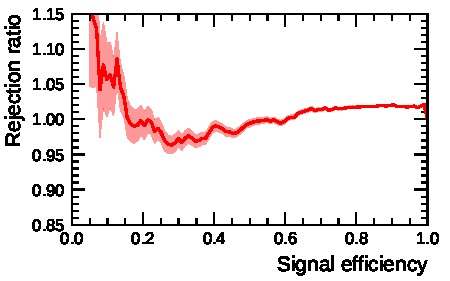
\includegraphics{./figures/rnn/mlp/mlp_bdt_ratio_1p.pdf}
    \subcaption{1-prong}
  \end{subfigure}\hfill
  \begin{subfigure}[t]{0.48\textwidth}
    \centering
    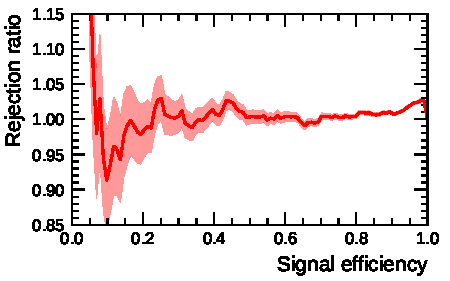
\includegraphics{./figures/rnn/mlp/mlp_bdt_ratio_3p.pdf}
    \subcaption{3-prong}
  \end{subfigure}
  \caption{Ratio of background rejection of the MLP and the optimised BDT as a
    function of signal efficiency. The band indicates the $1\sigma$-interval.}
  \label{fig:roc_mlp_bdt_comparison}
\end{figure}

Both the 1- and 3-prong MLP achieve similar performance characteristics as the
optimised BDT from Chapter~\ref{sec:bdt}, while requiring little optimisation of
the model hyperparameters. Therefore, neural networks are shown to be a viable
method of performing tau identification.

\section{Identification using Recurrent Neural Networks}
\label{sec:rnn_id}

Thus far approaches of tau identification use high-level variables that
summarise properties of reconstructed objects in the detector. This has the
advantage that identification can be understood and investigations into
systematic errors are simplified. However, discriminative power can be lost when
transitioning from low- to high-level variables. Therefore an approach is
presented capturing low-level information by employing sequence classification
techniques. A general description of the method is given and subsequently
applied to reconstructed tracks and clusters in the calorimeter.

\subsection{Motivation and General Description}
\label{sec:rnn_descr}

The variable importance of the BDT-based tau identification in
Section~\ref{sec:bdt_var_importance} shows that a large fraction of background
rejection can be attributed to variables derived from tracking information.
Examples are the variables sensitive to the decay length of the tau
lepton~$|S_\text{leadtrack}|$ and~$S_\text{T}^\text{flight}$ as well as the
transverse momentum fraction of isolation tracks~$f_\text{iso}^\text{track}$ and
the invariant mass of the track system~$m_\text{track}$. Moreover, during the
preparation of the tau identification for the ATLAS reconstruction release to be
used for the remainder of Run-II, it was observed that tracks classified as
\emph{isolation} offer discriminative power against \tauhadvis candidates from
multijet events. However, instabilities of the \emph{isolation} track category
lead to the necessity to decouple tau identification and the track
classification by introducing the \emph{modified isolation} category. This lead
to an average rejection loss of the order of \SI{20}{\percent} for the 1-prong
identification, while the 3-prong identification was not significantly affected.
Therefore, the aim is to improve the use of isolation information in
reconstructed tracks of \tauhadvis candidates.

For this purpose recurrent neural networks using the LSTM architecture are used
to classify a sequence of objects reconstructed in the detector. The following
will focus on describing the method using tracks in the ID but the use of other
physics objects is analogous. Figure~\ref{fig:track_rnn_schematic} describes the
architecture used in this chapter. Reconstructed \tauhadvis have a number of
associated tracks, which can be interpreted as elements in a sequence. Each
track in the sequence has variables related to the properties of the track,
e.g.\ the transverse momentum of the track. Moreover, the elements can also be
assigned global information about the \tauhadvis candidate like its visible
transverse momentum. The sequence of tracks is sorted according to a
well-defined and physically motivated ordering scheme. For the RNN using track
information a descending~$p_\text{T}^\text{track}$ ordering is used. In practice
the maximum sequence length is limited by truncation.

\begin{figure}[htb]
  \centering
  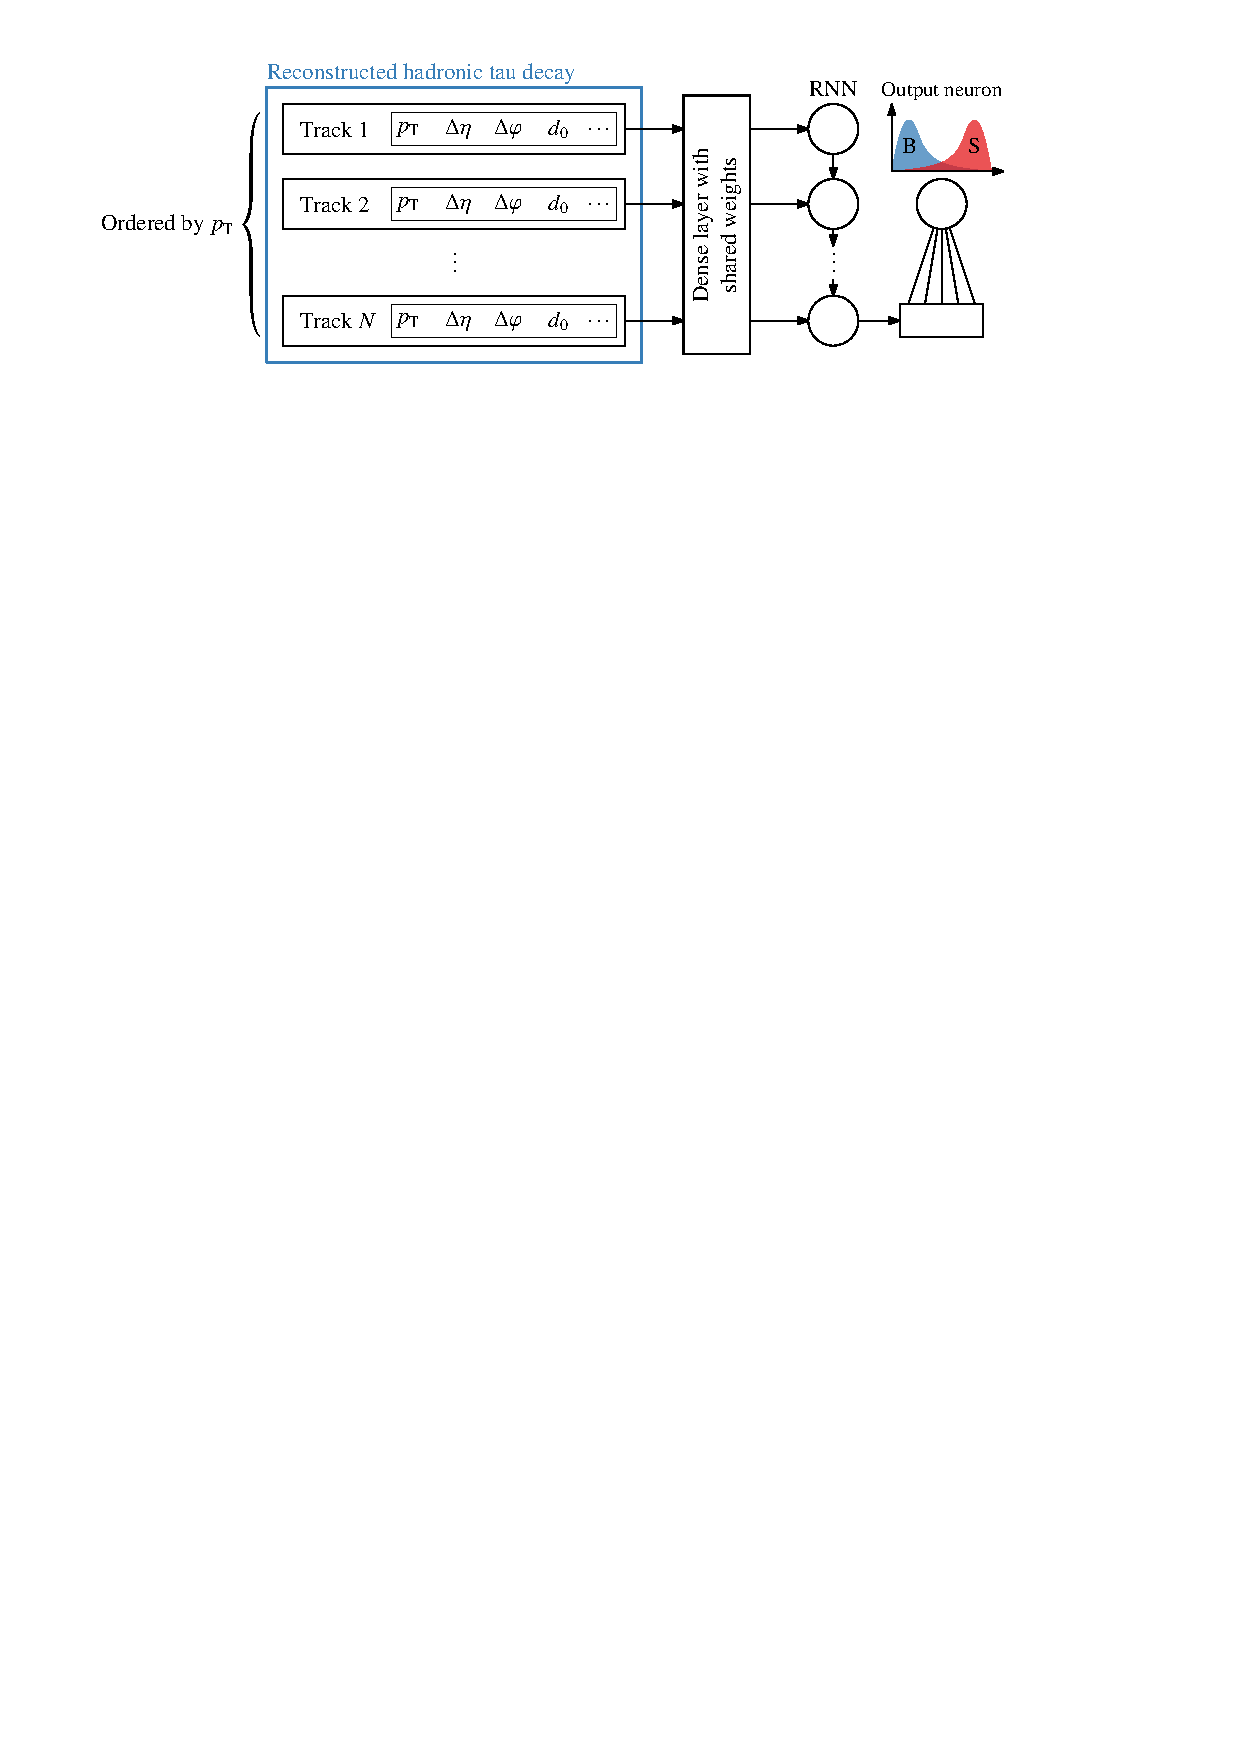
\includegraphics[scale=0.9]{./figures/rnn/track_rnn_schematic.pdf}
  \caption{Schematic description of a recurrent neural network using individual
    tracks for tau identification.}
  \label{fig:track_rnn_schematic}
\end{figure}

The tracks are passed in the predefined order to a dense layer with shared
weights. This layer applies a transformation on the input variables of each
individual track, where the trainable parameters of this transformation are
shared between each element in the sequence. It creates a sequence of
intermediate track representations, which are then passed to the recurrent layer
employing the LSTM architecture. The output of the final time step of the RNN,
consisting of a vector of activations, is passed to a dense layer with one
neuron and logistic sigmoid activation. The activation of the output neuron can
then be used to classify the \tauhadvis candidate as signal or background. The
intermediate layers use the hyperbolic tangent activation function.

\subsection{Network using Reconstructed Tracks in the Inner Detector}
\label{sec:rnn_tracks}

The implementation of the RNN employing track information, hereafter abbreviated
as Track--RNN, uses tracks associated with a \tauhadvis, which are tracks in
the~$\Delta R < 0.4$ cone with respect to the tau axis passing a transverse
momentum threshold of \SI{400}{\MeV} from track reconstruction. The variables
attached to each track are summarised in the following:
\begin{description}
\item[Transverse momentum of track and jet] The transverse momentum of the
  track~$p_\text{T}^\text{track}$ as measured in the tracking system is used.
  The inclusion of the track momentum is crucial as it allows the network to
  discriminate between tracks originating from the hard scattering and soft
  processes. Additionally, the transverse momentum of the anti-$k_\text{t}$ jet
  used to seed the \tauhadvis candidate~$p_\text{T}^\text{jet}$ is included in
  the input variables of each track. This allows tracks to be processed
  differently depending on the transverse momentum of the jet seed.

\item[Impact parameters] Information on the impact parameters of the track with
  respect to the associated primary vertex is included. The transverse impact
  parameter~$d_0$ is used directly, while the longitudinal impact parameter is
  included as~$z_0 \sin\theta$, where~$\theta$ is the polar angle of the track
  parametrisation.
  % This form accounts for larger errors of~$z_0$ for tracks in the forward
  % region.
  Impact parameter information is important to determine whether a given track
  originated from the tau production vertex. It allows to discriminate between
  tracks from the \tauhad or quark-/gluon-initiated jets and tracks from other
  interactions during the same bunch crossing.

\item[Angular distance to the tau axis] The signed angular distance of the track
  to the tau axis in the transverse~$\Delta \varphi$ and longitudinal
  direction~$\Delta \eta \coloneqq \eta_\text{track} - \eta_\tau$. The transverse
  angular distance~$\Delta \varphi$ is defined analogously to the longitudinal
  case but also accounting for the periodicity in the azimuthal angle~$\varphi$.
  The angular distances allow probing the spacial isolation of the tracks in a
  \tauhadvis candidate.

\item[Track quality criteria] The Track--RNN includes basic track quality
  criteria to allow to reject tracks of low reconstruction quality. For this the
  number of hits in the pixel layers~$N_\text{pixel}$ and semiconductor
  tracker~$N_\text{SCT}$ are used.
  % IBL TOO!

\item[Electron probability] The probability of the track originating from an
  electron estimated by a likelihood-based discriminant using high-threshold hit
  information in the TRT~$p_\text{HT}$. It is used to identify tracks
  originating from electrons created in photon conversion.
\end{description}
Including the track category from the multivariate track classification was also
investigated leading to a small improvement in discrimination power. It is not
included to keep the tau identification largely independent of track
classification.

Basic transformations are applied to the input variables to make them suitable
for use in neural networks. Therefore, a logarithm is applied to transverse
momenta~$p_\text{T}^\text{track}$, $p_\text{T}^\text{jet}$ and to the absolute
values of the impact parameters. Similar to the MLP, the input variables have to
be standardised. For transverse momenta and impact parameters this is done by
subtracting an offset and dividing by a scale factor. The offset is the mean of
the corresponding quantity in tracks of the training sample and the scale factor
the standard deviation. Signed angular distances are scaled into the
$[-1, 1]$-interval and similarly the number of hits in the ID into~$[0, 1]$. The
training process is analogous the the MLP and not repeated here.

The layer sizes in the architecture depicted in
Figure~\ref{fig:track_rnn_schematic} are optimised by observing the validation
loss while varying the number of units in different layers. A configuration
using 32 units in the shared dense layer and 32 units in the LSTM layer shows
good classification performance, while still being trainable in a moderate
amount of time. Alternative architectures using bidirectional LSTM and multiple
consecutive LSTM layers were investigated and show only marginal improvements
over the simpler model.

\todo[inline]{Continue}

In Figure~\ref{fig:ntracks_tau} the number of tracks associated to a given
\tauhadvis candidate is depicted. The number of associated tracks can be large,
especially for candidates from background events. For practical purposes the
sequence of tracks is truncated to reduce the memory footprint as well as
training and evaluation time of the network. As the tracks are sorted using a
descending $p_\text{T}^\text{track}$-ordering, truncation will only discard low
momentum tracks. Figure~\ref{fig:ntracks_loss} shows the classification power
for different number of tracks used in the model. The leading six tracks show a
significant impact on the discriminative power of the model. After ten tracks no
further improvement is observed. Therefore, the model will use tracks truncated
after the ten leading tracks in transverse track momentum.

\begin{figure}[htb]
  \begin{subfigure}[t]{0.48\textwidth}
    \centering
    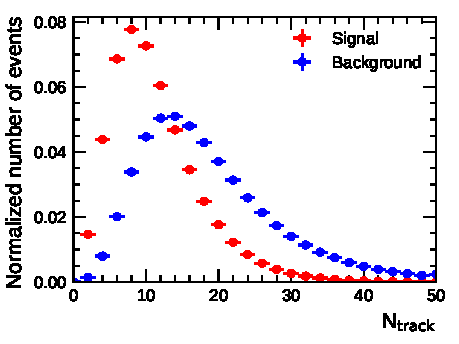
\includegraphics{./figures/rnn/ntrk_1p.pdf}
    \subcaption{Number of tracks associated to a reconstructed 1-prong tau
      candidate.}
    \label{fig:ntracks_tau}
  \end{subfigure}\hfill
  \begin{subfigure}[t]{0.48\textwidth}
    \centering
    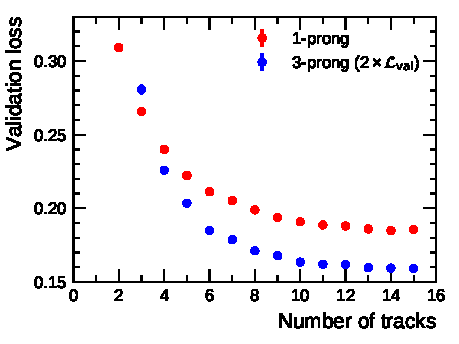
\includegraphics{./figures/rnn/nscan/track_1p_3p.pdf}
    \subcaption{Validation loss as a function of the number of tracks used in
      the model.}
    \label{fig:ntracks_loss}
  \end{subfigure}
  \caption{Number of tracks associated to a \tauhadvis candidate and their
    impact on the discriminative power of the Track--RNN.}
  \label{fig:rnn_ntracks}
\end{figure}

A comparison of the ROC-curves for the BDT- and RNN-based tau identification is
depicted in Figure~\ref{fig:track_rnn_roc_ratios}. Both the 1- and 3-prong
Track--RNN show a performance similar to the optimised BDT. The 1-prong
Track--RNN shows a small improvement in rejection of \num{10} to
\SI{20}{\percent} over the BDT depending on the signal efficiency. In contrast
to this the 3-prong RNN cannot exceed the performance of the optimised BDT, only
capturing \num{80} to \SI{90}{\percent} of rejection. These results indicate
that the available information in tracks is not fully exploited in the current
BDT-based identification.

\begin{figure}[htb]
  \begin{subfigure}[t]{0.48\textwidth}
    \centering
    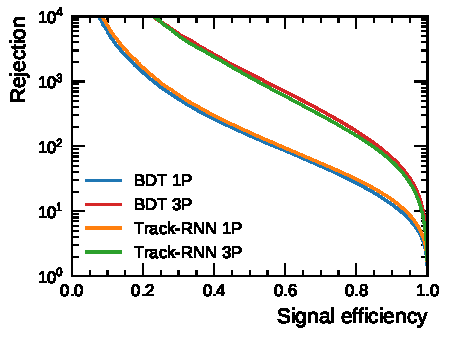
\includegraphics{./figures/rnn/track/roc.pdf}
    \subcaption{ROC-curves for 1-prong (1P) and 3-prong (3P) tau
      identification.}
  \end{subfigure}\hfill
  \begin{subfigure}[t]{0.48\textwidth}
    \centering
    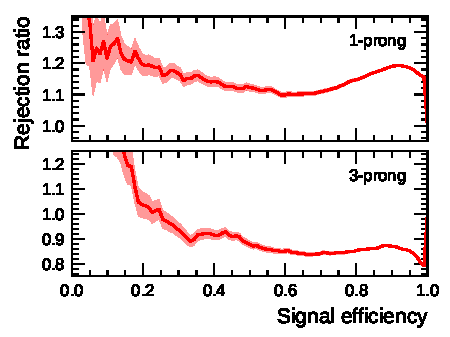
\includegraphics{./figures/rnn/track/ratios.pdf}
    \subcaption{Ratio of rejection of the Track--RNN and the optimised BDT. The
      band indicates the $1\sigma$-interval.}
  \end{subfigure}
  \caption{Classification performance of the Track--RNN compared to the
    optimised BDT for tau identification.}
  \label{fig:track_rnn_roc_ratios}
\end{figure}

Due to the complexity of the network, interpretation of the model based on the
parameters learned during training is not possible. It must be viewed as a black
box where only the input and the output can be accessed. Nevertheless the
variable importance and linear correlations of output and inputs can be
evaluated to gain a better understanding of the model. In
Table~\ref{tab:var_importance_track_rnn} the importance of the inputs is
estimated by removing groups of related variables and retraining the model. The
increase in validation loss is used to rank the importance of the input
variables. The table shows that the impact parameters and transverse momenta
have a large impact on the loss. They are essential to identify tracks
originating from the hard scattering as opposed to tracks from other
interactions or pile-up. The angular distances~$\Delta \eta$
and~$\Delta \varphi$ show an importance similar to the transverse momenta.
Compared to multijet events, tracks from hadronic tau decays are expected to be
close to the tau axis resulting in small angular distances for tracks
originating from the tau. The number of hits in the ID and the electron
probability~$p_\text{HT}$ shows only a marginal importance in the Track--RNN.

\begin{table}[htb]
  \centering
  {\small\begin{tabular}{p{5cm}S[table-format=1.4(4)]S[retain-explicit-plus, table-format=+2.1]}
  \toprule
  {Variables} & {Validation loss} & {Loss increase} \\
  \midrule
  \parbox[c]{\hsize}{Impact parameter \newline $d_0$, $z_0 \sin\theta$}
          & 0.2831 +- 0.0005 & + 48.4 \,\si{\percent} \\[1.2em]
  \parbox[c]{\hsize}{Transverse momentum \newline $p_\text{T}^\text{track}$, $p_\text{T}^\text{jet}$}
          & 0.2410 +- 0.0007 & + 26.3 \,\si{\percent} \\[1.2em]
  \parbox[c]{\hsize}{Angular distance \newline $\Delta \eta$, $\Delta \varphi$}
          & 0.2304 +- 0.0003 & + 20.8 \,\si{\percent} \\[1.2em]
  \parbox[c]{\hsize}{Hits in ID \newline $N_\text{hit}^\text{pixel}$, $N_\text{hit}^\text{SCT}$}
          & 0.2036 +- 0.0013 & + 6.7 \,\si{\percent} \\[1.2em]
  \parbox[c]{\hsize}{Electron probability (TRT) \newline $p_\text{HT}$}
          & 0.1930 +- 0.0004 & + 1.2 \,\si{\percent}\\
  \bottomrule
\end{tabular}

%%% Local Variables:
%%% mode: latex
%%% TeX-master: "../mythesis"
%%% End:
}
  \caption{Variable importance of the 1-prong Track--RNN estimated by the
    increase in validation loss when removing groups of input variables.}
  \label{tab:var_importance_track_rnn}
\end{table}

In Figure~\ref{fig:track_rnn_correlations} the correlations of the input
variables for each track in the sequence with the signal
probability~$p_\text{RNN}$ estimated by the Track--RNN is depicted. In hadronic
tau lepton decays the leading tracks in transverse momentum often correspond the
to the charged decay products. This can be seen in the significant change in
correlation after the first or first three tracks for 1- and 3-prong candidates,
respectively. The correlation of the transverse track
momentum~$p_\text{T}^\text{track}$ in Figure~\ref{fig:track_rnn_corr_pt} shows a
positive coefficient for the leading tracks. The positive correlation implies
that candidates with leading tracks with high transverse momentum are more
likely to get assigned a large signal probability~$p_\text{RNN}$ by the model.
In contrast to this, subleading tracks with large transverse momentum tend to
reduce the signal probability, thus are more likely associated with background
\tauhadvis candidates. Similarly, the distance of closest approach to the
primary vertex in the $\rho z$-plane~$|z_0 \sin\theta|$ in
Figure~\ref{fig:track_rnn_corr_z0} shows that signal candidates are more likely
to have leading tracks close to the primary vertex, while subleading tracks
exhibit larger distances to the vertex. The same behaviour is observed for the
transverse impact parameter~$|d_0|$ and the $\Delta R$-distance to the tau axis,
which can be calculated using the signed angular distances~$\Delta \eta$ and
$\Delta \varphi$.

\begin{figure}[htb]
  \centering
  \begin{subfigure}[t]{0.48\textwidth}
    \centering
    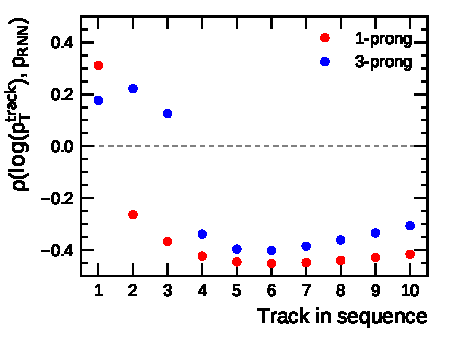
\includegraphics{./figures/rnn/track/pt_corr.pdf}
    \subcaption{Transverse momentum of the track~$p_\text{T}^\text{track}$.}
    \label{fig:track_rnn_corr_pt}
  \end{subfigure}\hfill
  \begin{subfigure}[t]{0.48\textwidth}
    \centering
    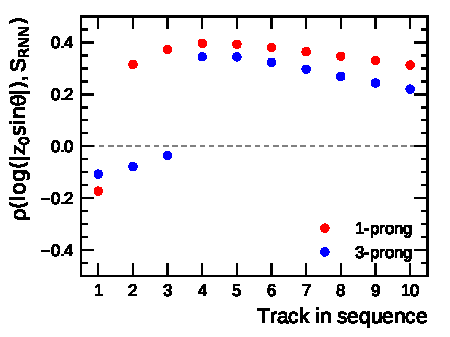
\includegraphics{./figures/rnn/track/z0_corr.pdf}
    \subcaption{Distance of closest approach to the primary vertex in the
      $\rho z$-plane~$|z_0 \sin\theta|$.}
    \label{fig:track_rnn_corr_z0}
  \end{subfigure}
  \caption{Linear correlation coefficient between input variables and signal
    probability~$p_\text{RNN}$ estimated by the model. The coefficient is
    determined on the testing sample combining signal and background candidates
    with equal total weight.}
  \label{fig:track_rnn_correlations}
\end{figure}

\todo[inline]{Write transition paragraph? Working points deferred to later.}

\subsection{Network using Clusters in the Calorimeter System}
\label{sec:rnn_clusters}

The BDT-based tau identification makes extensive use of calorimetric information
using cluster of calorimeter cells created by the TopoCluster algorithm and
other quantities calculated from cells in the calorimeter system. Therefore, a
separate network is developed employing TopoClusters associated with the jet
seeding a \tauhadvis candidate, hereafter called the Cluster--RNN. The variable
selection is given in the following:
\begin{description}
\item[Transverse energy/momentum] The transverse energy of the
  cluster~$E_\text{T}$ and the transverse momentum of the jet seeding the
  \tauhadvis candidate~$p_\text{T}^\text{jet}$ is used. The motivation for
  including these variables is analogous to the Track--RNN.

\item[Angular distance to the tau axis] The signed angular distance of the
  cluster barycentre to the tau axis in the longitudinal~$\Delta \eta$ and
  transverse plane~$\Delta \varphi$.

\item[Cluster and signal moments] Identification variables like the central
  energy fraction~$f_\text{cent}$ use quantities calculated from individual
  cells in the calorimeter. Cell-level information is not available in the
  samples used for this study. Therefore, cluster and signal moments of the
  TopoClusters are used to obtain information on cluster shape and energy
  density.

  The moments used for the Cluster--RNN are summarised in the following. The
  lateral shower width~$\langle R^2 \rangle$ given by the second moment of the
  radial distance~$R$ between cluster cells and shower axis. The longitudinal
  shower width~$\langle \lambda^2 \rangle$ with the distance~$\lambda$ of cells
  from the barycentre of shower energy measured along the shower axis. The depth
  of the shower centre~$\lambda_\text{centre}$ measured from the face of the
  calorimeter. Finally, the mean energy density~$\langle \rho \rangle$ and
  energy fraction of the most energetic cell~$f_\text{max}$ is used. These
  cluster and signal moments are calculated by the TopoCluster
  algorithm~\cite{atlas_topoclustering}.
\end{description}
Additionally, energy fractions of clusters in the different samplings of the
electromagnetic calorimeter and the probability of a cluster originating from an
electromagnetic
shower~$\mathcal{P}_\text{clus}^\text{EM}$~\cite{atlas_topoclustering}, which is
used in the local hadronic calibration, are investigated. These variables are
not found to improve the classification power of the cluster-based
identification.

The input variables are transformed and standardised similar to the track-based
identification. The cluster moments are log-transformed and standardised by
subtracting an offset and dividing by a scale factor. The signal
moment~$f_\text{max}$ does not require preprocessing. The remaining variables
are processed in analogy to the Track--RNN.

The architecture used for the Cluster--RNN is identical to the one used for the
Track-RNN. However, the number of units in the LSTM layer is reduced to 24 (from
32), while the shared dense layer remains at 32 units. Clusters are passed in
ascending $E_\text{T}$-ordering to the network. Figure~\ref{fig:rnn_nclusters}
shows the number of clusters in the jet used to seed the \tauhadvis candidate
and the impact of truncating the cluster sequence on the validation loss. The
cluster-based identification shows no improvement in classification power after
the six leading clusters in~$E_\text{T}$. Therefore, only the six leading
clusters of the jet seed are used for tau identification using the Cluster--RNN.

\begin{figure}[htb]
  \begin{subfigure}[t]{0.48\textwidth}
    \centering
    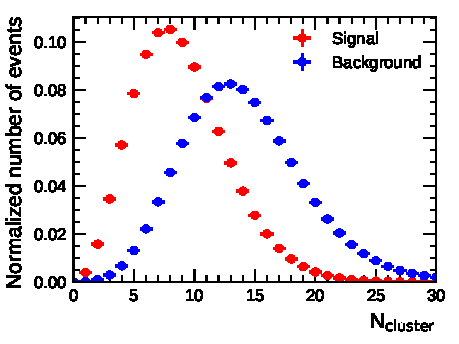
\includegraphics{./figures/rnn/ncls_1p.pdf}
    \subcaption{Number of clusters in the anti-$k_\text{t}$ jet used to seed the
      1-prong \tauhadvis candidates.}
  \end{subfigure}\hfill
  \begin{subfigure}[t]{0.48\textwidth}
    \centering
    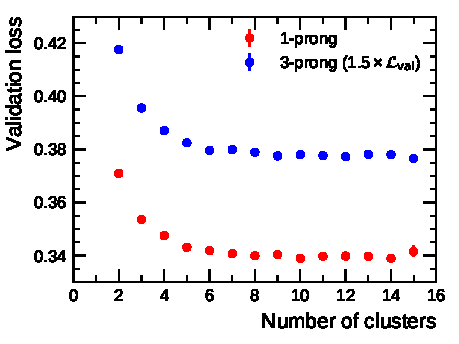
\includegraphics{./figures/rnn/nscan/cluster_1p_3p.pdf}
    \subcaption{Validation loss as a function of the number of clusters used in
      the model.}
  \end{subfigure}
  \caption{Number of clusters associated to a \tauhadvis candidate and their
    impact on the discriminative power of the Cluster--RNN.}
  \label{fig:rnn_nclusters}
\end{figure}

The classification performance after training the model for 1- and 3-prong
\tauhadvis candidates separately is shown in
Figure~\ref{fig:cluster_rnn_roc_ratios}. The 1- and 3-prong Cluster--RNN show
similar performance characteristics. However, the purely cluster-based
identification cannot reach performances comparable to the tau identification
using the optimised BDT. For the identification of 1-prong \tauhadvis the
rejection \num{10} to \SI{40}{\percent} depending on the signal efficiency. Due
to the large rejection of the 3-prong BDT-based identification the Cluster--RNN
can only reach \num{2} to \SI{10}{\percent} of the full rejection.

\begin{figure}[htb]
  \begin{subfigure}[t]{0.48\textwidth}
    \centering
    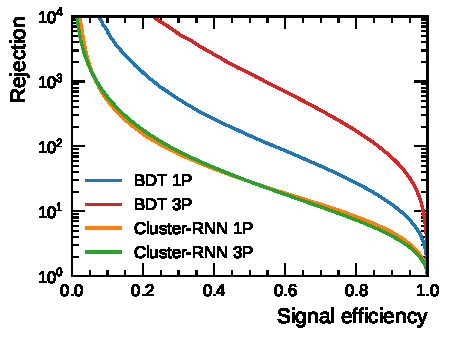
\includegraphics{./figures/rnn/cluster/roc.pdf}
    \subcaption{ROC-curves for 1-prong (1P) and 3-prong (3P) tau
      identification.}
  \end{subfigure}\hfill
  \begin{subfigure}[t]{0.48\textwidth}
    \centering
    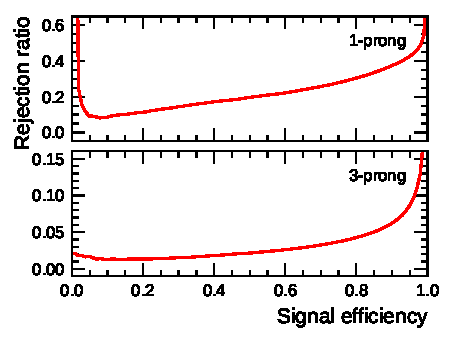
\includegraphics{./figures/rnn/cluster/ratios.pdf}
    \subcaption{Ratio of rejection of the Cluster--RNN and the optimised BDT.}
  \end{subfigure}
  \caption{Classification performance of the Cluster--RNN compared to the
    optimised BDT for tau identification.}
  \label{fig:cluster_rnn_roc_ratios}
\end{figure}

The most important variables for the operation of the Cluster--RNN are the
angular distances~$\Delta \eta$ and~$\Delta \varphi$ followed by the
$E_\text{T}$ of the cluster and the transverse momentum of the jet
seed~$p_\text{T}^\text{jet}$. The cluster and signal moments, while still
contributing significantly to the discriminative power, are the least important.
This variable ranking indicates that a significant part of the discriminative
power is obtained by requiring isolated showers close to the tau axis.

Due to the small rejection, the standalone operation of the Cluster--RNN is not
of interest to the offline reconstruction of \tauhadvis. However, it can
potentially be used for \tauhadvis identification at trigger-level, where track
and vertex reconstruction is infeasible due to time constraints.

\subsubsection{Online Di-Tau Identification at the High Luminosity LHC}
\label{sec:hlt_rate_reduction}

The Phase-II upgrade of the LHC called the High Luminosity LHC (HL-LHC) is
foreseen to be finished by 2026. It will increase the instantaneous luminosity
to~\num{5}\,--\,\SI{7.5e34}{\per\square\centi\metre\per\second} at a
centre-of-mass energy
of~$\sqrt{s} = \SI{14}{\TeV}$~\cite{hl_lhc_prelim_design_report}. This
corresponds to a five- to sevenfold increase in luminosity with respect to the
beginning of Run-II and increases the average number of interactions per bunch
crossing to up to \num{200}. The increase in particle density poses a challenge
to the trigger systems and reconstruction algorithms.

An upgrade of the ATLAS trigger with a \emph{Global Trigger System} aims to
provide access to the full calorimeter granularity with topoclustering and jet
finding using iterative jet algorithms in regions of
interest~\cite{phase_2_scoping}. This aims to improve the identification of
physics objects at trigger-level to cope with increasing trigger rates due to
pile-up. Due to the availability of full calorimeter granularity, offline
reconstructed \tauhadvis can be used to give prospects of the potential
performance of triggers for \tauhadvis in the HL-LHC environment.

A prospective study focusing on the usage of the cluster-based RNN for
identification of \tauhadvis in a di-tau trigger is given. Offline \tauhadvis
are used as an approximation to reconstructed taus at trigger-level after the
Phase-II upgrade. The study uses simulated samples
of~$\text{Z} / \text{DY} \to \tau \tau$ and dijets at HL-LHC conditions with
centre-of-mass energy~$\sqrt{s}=\SI{14}{\TeV}$ and average interactions per
bunch crossing~$\mu = 200$ (cf.\ Appendix~\ref{app:upgrade_samples}).

The cluster-based RNN identification is retrained on \tauhadvis candidates of
the HL-LHC upgrade samples using the same preselection used for the BDT
identification in Chapter~\ref{sec:bdt} with the exception of any
tracking-related requirements. The leading and subleading \tauhadvis with
respect to the reconstructed transverse momentum (using Run-II calibrations) are
selected in a given event, while additionally requiring a truth-matched hadronic
tau decays for the signal sample. The RNN identification is applied to each
\tauhadvis individually resulting in two identification scores per event. The
leading and subleading \tauhadvis~$p_\text{T}$ and identification scores are
combined in a logistic regression to assign a single di-tau identification score
to each event.

The accept-rate of \SI{200}{\kilo\hertz} of the higher-level triggers limits the
maximum trigger rate of the di-tau trigger. Achieving this rate requires
$p_\text{T}$-thresholds on leading and subleading \tauhadvis as well as
application of the di-tau identification. The thresholds should be kept low to
ensure high signal acceptance for physics analyses. For the purposes of this
study a single cut on the identification score is used to identify di-tau
events.

\begin{figure}[htb]
  \centering
  \begin{subfigure}[t]{0.48\textwidth}
    \centering
    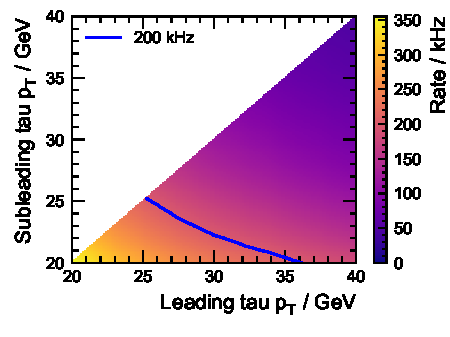
\includegraphics{./figures/rnn/trigger/pt_rate_reg.pdf}
    \subcaption{Trigger-rate after RNN-based identification as a function of
      leading and subleading tau offline $p_\text{T}$-threshold.}
    \label{fig:rate_vs_thresholds}
  \end{subfigure}\hfill
  \begin{subfigure}[t]{0.48\textwidth}
    \centering
    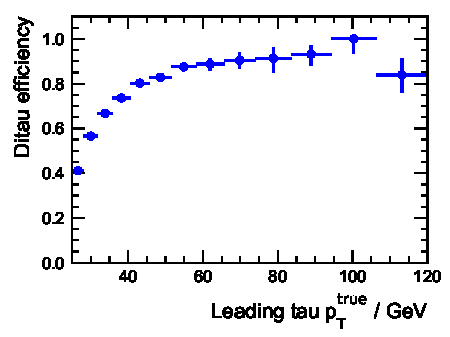
\includegraphics{./figures/rnn/trigger/taueff_reg.pdf}
    \subcaption{Di-tau selection efficiency of RNN-based identification with
      \SI{25}{\GeV} $p_\text{T}$-thresholds with respect to offline
      reconstructed tau lepton pairs measured in $\text{Z} \to \tau\tau$.}
    \label{fig:ditau_trigger_eff}
  \end{subfigure}
  \caption{Feasibility of using TopoClusters for a di-tau trigger at the
    HL-LHC.}
  \label{fig:rnn_ditau_trigger}
\end{figure}

Due to the large dijet production cross section it is assumed, that the
background events in the simulated sample correspond to a trigger rate equal to
the average bunch crossing rate of~\SI{31.6}{\mega\hertz}. In
Figure~\ref{fig:rate_vs_thresholds} the trigger-rate is shown as a function of
the leading and subleading \tauhadvis $p_\text{T}$-thresholds after applying
di-tau identification. The target rate can be achieved with a offline
$p_\text{T}$-threshold of \SI{25}{\GeV} on both \tauhadvis candidates.
Figure~\ref{fig:ditau_trigger_eff} shows the efficiency of the identification
using the leading and subleading \SI{25}{\GeV} threshold with respect to all
offline reconstructed di-tau events. The di-tau efficiency starts to plateau at
true visible transverse momentum~$p_\text{T}^\text{true} > \SI{40}{\GeV}$ of the
leading \tauhadvis with an efficiency of approximately~\SI{90}{\percent}.

Ref.~\cite{phase_2_scoping} outlines a di-tau trigger with offline
$p_\text{T}$-threshold on the leading and subleading tau of \SI{40}{\GeV} and
\SI{30}{\GeV}, respectively. The approach using the cluster-based RNN
identification achieves the target rate at a reduced $p_\text{T}$-threshold
of~\SI{25}{\GeV}. The efficiency of the selection shows opportunities for
further enhancements by employing a proper tau energy calibration for HL-LHC
conditions and using a more advanced decision threshold for the di-tau
identification. The decision threshold could be loosened with increasing
transverse momentum to ensure a quicker turn-on and full efficiency at
high-$p_\text{T}$.

\subsection{Combined Network}
\label{sec:rnn_combined}

After introducing the MLP using the high-level identification variables, the
track-based RNN and the cluster-based RNN, a network combining these models is
trained. An improvement in rejection is expected when combining the models,
although a large fraction of information will be redundant.

The architecture of the combined model builds on the previously developed MLP,
Track--RNN and Cluster--RNN architectures. A schematic description of the
architecture is given in Figure~\ref{fig:schematic_combined}. The combined model
contains three distinct branches. The branches using track and cluster inputs
are inherited from the Track-- and Cluster-RNN, respectively. The sizes of the
shared dense and LSTM layers are unchanged. The third branch is derived from the
MLP using high-level identification variables. While the first two layers of the
MLP are unchanged, a third dense layers with 16 units is added. The three
branches are combined into a single output by merging their outputs in a final
dense layer.

\begin{figure}[htb]
  \centering
  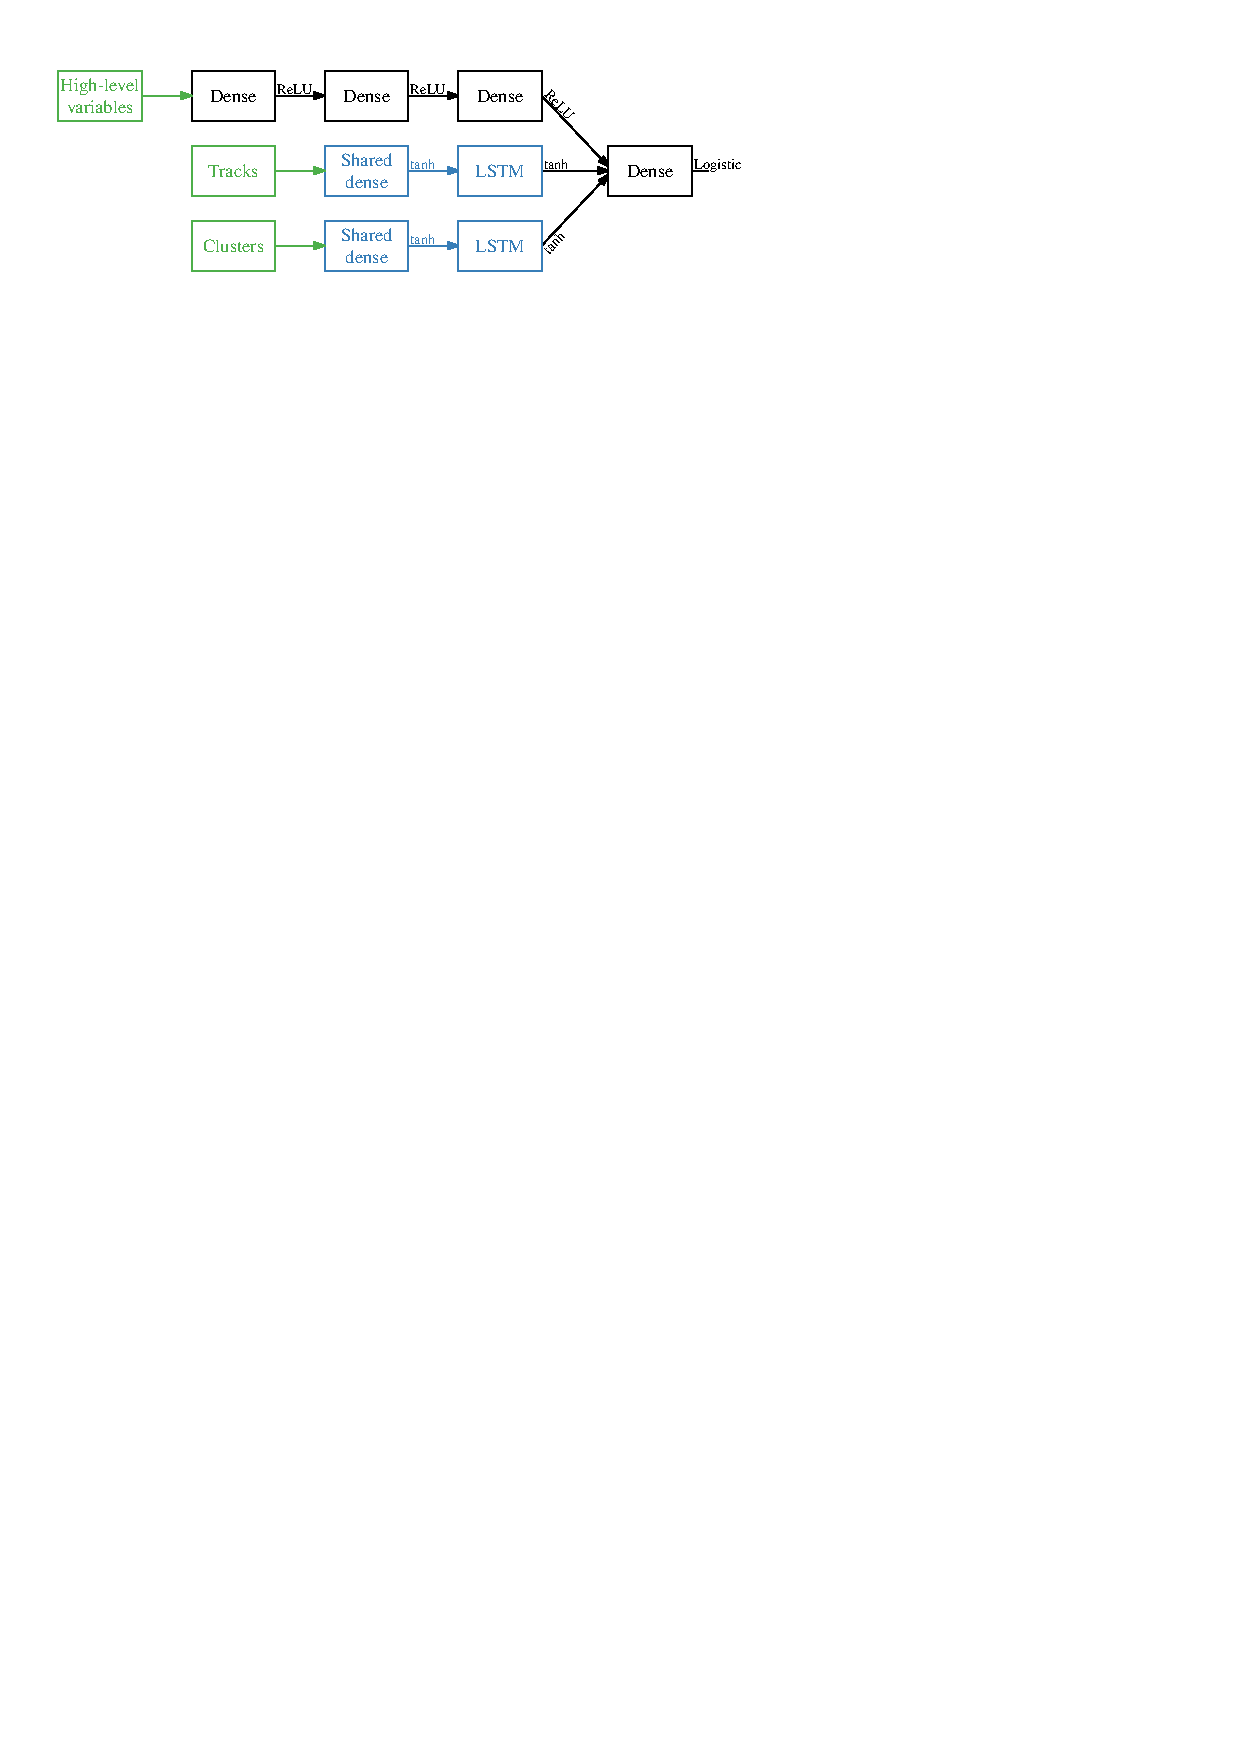
\includegraphics{./figures/rnn/combined_architecture.pdf}
  \caption{Architecture of the combined model operating on high-level
    identification variables and sequences of tracks and clusters. The
    activation function is denoted after each layer (cf.\ Chapter~\ref{sec:ml}).
    Layers operating on sequential inputs are highlighted in blue.}
  \label{fig:schematic_combined}
\end{figure}

Figure~\ref{fig:roc_combined} compares the ROC-curves of the combined model and
the optimised BDT of Chapter~\ref{sec:bdt}. A model combining MLP and Track--RNN
without including the Cluster--RNN is also shown. The combined model shows a
significant improvement on the BDT-based tau identification. The background
rejection is increased by a factor of two for 1-prong and approximately
\SI{50}{\percent} for 3-prong candidates. The contribution of the cluster
information to the rejection is small with an improvement of approximately
\SI{10}{\percent} over a model omitting the cluster branch. This allows to
simplify the model without incurring a large loss in discriminative power.
\todo{Write sth.\ about Track+Cluster}

\begin{figure}[htb]
  \begin{subfigure}[t]{0.48\textwidth}
    \centering
    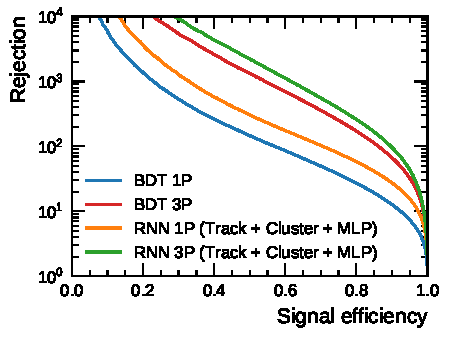
\includegraphics{./figures/rnn/combined/roc.pdf}
    \subcaption{ROC-curves for 1-prong (1P) and 3-prong (3P) tau identification.}
  \end{subfigure}\hfill
  \begin{subfigure}[t]{0.48\textwidth}
    \centering
    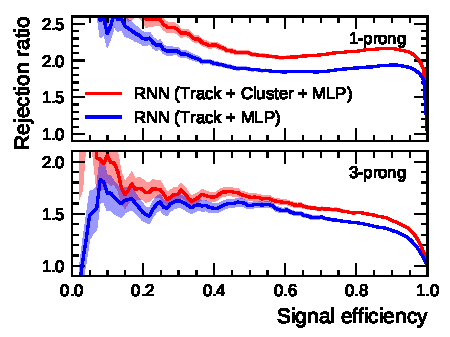
\includegraphics{./figures/rnn/combined/ratios.pdf}
    \subcaption{Ratio of rejection of the combined model and the optimised BDT.}
  \end{subfigure}
  \caption{Classification performance of the combined model compared to the
    optimised BDT for tau identification.}
  \label{fig:roc_combined}
\end{figure}

The background rejection of the tight working point for the 1- and 3-prong tau
identification using the RNN is shown in
Figure~\ref{fig:combined_working_points} and compared with the BDT-based
identification from Chapter~\ref{sec:bdt}. The combined model shows a relative
increase in rejection of the tight working point ranging from \SI{70}{\percent}
to \SI{150}{\percent} for 1-prong and \SI{40}{\percent} to \SI{100}{\percent}
for 3-prong tau identification over the optimised BDT-based model. In both cases
an increase in background rejection with increasing \tauhadvis \pt is observed.
A possible explanation for this behaviour is an enhanced capability of the RNN
to identify tracks originating from quark- or gluon-initiated jets. Ultimately,
this is because the track classification is optimised to reconstruct \tauhadvis
originating from hadronic tau decays with the correct number of tracks, whereas
it does not claim to reconstruct \tauhadvis from quark- or gluon-initiated jets
with the correct charged-particle multiplicity. The increasing charged-particle
multiplicity for high-\pt jets could therefore lead to an improved background
rejection. The medium and loose working points show similar improvements (cf.\
Appendix~\ref{app:rnn_wp}).

\begin{figure}[htb]
  \begin{subfigure}[t]{0.48\textwidth}
    \centering
    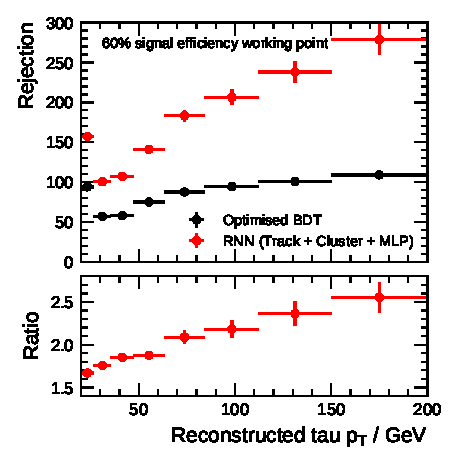
\includegraphics{./figures/rnn/combined/rnn_tight_1p.pdf}
    \subcaption{1-prong}
  \end{subfigure}\hfill
  \begin{subfigure}[t]{0.48\textwidth}
    \centering
    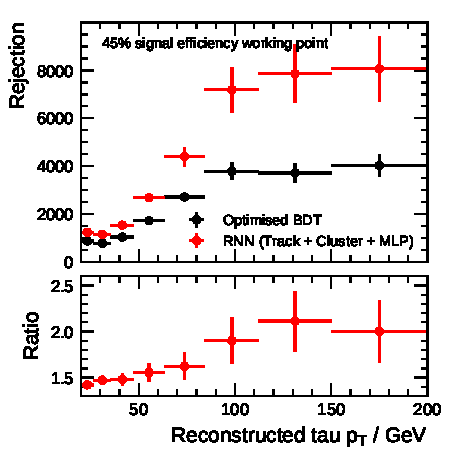
\includegraphics{./figures/rnn/combined/rnn_tight_3p.pdf}
    \subcaption{3-prong}
  \end{subfigure}
  \caption{Background rejection at the tight working point as a function of the
    reconstructed tau $p_\text{T}$ at tau energy scale for the BDT- and
    RNN-based identification.}
  \label{fig:combined_working_points}
\end{figure}

The improvements in background rejection allow to loosen the working points,
thus increasing the signal efficiency, while still maintaining a rejection
comparable to the nominal working point of the BDT-based identification. An
example is the efficiency of the tight working point for the 1-prong
identification, which can be increased from \SI{60}{\percent} to
\SI{70}{\percent}. In doing this the rejection of fake \tauhadvis candidates
with transverse momentum of \SI{20}{\GeV} matches the rejection of the BDT using
the nominal tight working point. For larger \tauhadvis \pt the rejection of the
RNN at the loosened working point still exceeds the BDT-based identification.
Analogously, the signal efficiency of the 3-prong tight working point can be
increased from \SI{45}{\percent} to \SI{50}{\percent}. A detailed comparison of
the background rejection of the loosened and nominal working point as a function
of \tauhadvis \pt is omitted for brevity and can be found in
Appendix~\ref{app:loosened_wp}.

Analyses requiring two \tauhadvis with tight identification in the reconstructed
final state, e.g.\ measurements in the~\mbox{$H \to \tauhad \tauhad$} channel,
can benefit from introducing working points with increased signal efficiency.
Assuming the identification scores of the \tauhadvis in the final state are
uncorrelated, a 1-prong working point with \SI{70}{\percent} signal efficiency
increases the number of signal events by \SI{36}{\percent} compared to the
nominal working point. Moreover, a 3-prong working point with \SI{50}{\percent}
signal efficiency improves the signal yield by \SI{23}{\percent}. The RNN-based
identification can achieve these working point efficiencies, while offering
rejection rates matching or exceeding the nominal working points of the
optimised BDT depending on the \tauhadvis momentum. For searches of additional
heavy neutral Higgs and gauge bosons~\cite{mssm_higgs_zprime}, where the
reconstructed final state is expected to contain \tauhadvis with high transverse
momenta, the working point efficiencies could be increased even further.
% 1-prong
% 0.6 * 0.6 = 0.36
% 0.7 * 0.7 = 0.49
% 0.49 / 0.36 = 1.3611111111 -> 36 % relative increase in signal
%
% 3-prong
% 0.45 * 0.45 = 0.2025
% 0.5 * 0.5 = 0.25
% 0.25 / 0.2025 = 1.234567901234568 -> 23 % relative increase in signal

This concludes the studies related to tau identification...

\todo[inline]{Whats with Track-RNN + Cluster-RNN?}

\todo[inline]{Have at least an exemplary RNN score in the appendix.}

\todo[inline]{Missing hits for taus decaying after pixel layers. Questionable
  modelling of impact parameters. Also number of hits is directly used. Should
  not affect low momentum taus. $p_\text{T} = \SI{200}{\GeV}$ taus -- less than
  \SI{5}{\percent} decay after the IBL.}

\todo[inline]{Pile-up dependency of RNN vs BDT-ID}

\todo[inline]{Regained lost rejection from modified isolation category.}

\todo[inline]{Some standard plots: Efficiency vs pt vs eta vs mu (same with rejection?)}

\todo[inline]{High pt rejection in appendix}

%%% Local Variables:
%%% mode: latex
%%% TeX-master: "mythesis"
%%% End:
